% TMLR anonymous review version. Official style files are unmodified.
\documentclass[10pt]{article}
\usepackage[utf8]{inputenc}
\usepackage{tmlr}
\usepackage{amsmath,amssymb}
\usepackage{graphicx}
\usepackage{pdflscape}
\usepackage{longtable,booktabs,array,calc}
\usepackage{url}
\usepackage[hidelinks]{hyperref}
\usepackage{bookmark}
\usepackage[nameinlink,noabbrev]{cleveref}
\usepackage{xurl}
\providecommand{\tightlist}{\setlength{\itemsep}{0pt}\setlength{\parskip}{0pt}}
\newcommand{\pandocbounded}[1]{#1}
\bibliographystyle{tmlr}
\hypersetup{pdfauthor={},pdftitle={Activation-Patching Measurements in CNNs Depend on Channel Budget, Architecture, and Spatial Prior Structure}}

\title{Activation-Patching Measurements in CNNs Depend on Channel Budget, Architecture, and Spatial Prior Structure}
\author{}
\date{}

\begin{document}
\maketitle

\begin{abstract}
Activation patching asks how a model output changes when internal activations are replaced, but the resulting measurement is conditional on how the intervention is defined. We study this problem in controlled convolutional networks whose first layer is initialized from a predefined bank of edge, corner, and ring filters. Constant regularization preserves this spatial structure, whereas an annealed condition releases the first layer during training. On exact matched counterfactual image pairs, a prospectively frozen test on 20 fresh renderer blocks shows that the release-versus-retention comparison changes sharply with the number of patched first-layer channels: the prespecified contrast between $k=4,8$ and $k=1,2$ is $B=0.33098$ (95\% CI $[0.27368,0.38827]$) under the historical probability metric. The same prespecified contrast remains positive under centered-logit fidelity and an unnormalized probability-error reduction, although their pointwise curves differ. A separate 100-block study across 16 CNN variants finds strong architecture heterogeneity under both primary metrics, and post hoc Greenhouse--Geisser, permutation, Friedman, and random-channel diagnostics preserve that conclusion. Finally, a fresh 25,600-model specificity experiment compares the original filters with a common pixel permutation that preserves the template-bank Gram matrix, rank, singular spectrum, row norms, and coefficient multisets. For validation-selected channels, spatial structure changes $B$ by $+0.05743$ in centered-logit fidelity and is not practically equivalent under a frozen margin; the probability-error difference is statistically nonzero but practically equivalent. The spatial effect also reverses sign in one downstream architecture and is much smaller for random channel sets. Thus weight-space structure, concentration of functional effects in selected channels, and activation-patching measurements are distinct quantities: conclusions in this setting depend on channel budget, downstream architecture, output metric, and spatial prior structure.\footnote{ChatGPT (OpenAI) was used as an assistive tool during experimental planning, code development and debugging, manuscript organization, and language editing. All experimental protocols, analyses, interpretations, and manuscript text were reviewed by the authors, who take full responsibility for the work.}
\end{abstract}

\section{Introduction}\label{sec:introduction}

The first convolutional layer is one of the few places in a vision network where learned weights can still be inspected directly as spatial filters. This has motivated a long line of work asking whether early spatial filters should be learned freely at all. Wavelet and Gabor constructions provide useful fixed image representations \citep{bruna_2013_scattering-networks}; Gabor initialization, maintained filter structure, learnable Gabor parameterizations, and predefined-filter networks impose stronger spatial priors on CNNs \citep{ozbulak_2018_gabor-initialization,molaei_2020_gabor-filter-structure,wang_2024_learnable-gabor,linse_2024_predefined-filters,orozco-solis_2024_learnable-gabor-filters}; and fixed or even random spatial kernels can remain effective when later layers learn how to recombine them \citep{gaudio_2023_fixed-filters,gavrikov_2023_random-convolutions}. Analyses of unconstrained CNNs likewise find regular first-layer frequency structure and sensitivity of early filters to training-data statistics \citep{chowers_2023_first-layer-filters,jorgenson26ajorgenson_2026_early-cnn-filters}. These results motivate structured first-layer priors, but they leave open a different question: if a first layer remains structurally close to an intended spatial basis, does that structure have a stable functional signature inside the trained network?

The distinction matters because representational alignment and functional influence are not interchangeable. Network Dissection, TCAV, Concept Whitening, concept bottlenecks, and related approaches measure or impose different forms of alignment between internal representations and human-defined concepts \citep{bau_2017_network-dissection,kim_2018_tcav,chen_2020_concept-whitening,koh_2020_concept-bottlenecks}. Subsequent work shows that apparently aligned representations can leak unintended information, fail to correspond to intended semantics, or dissociate from influence on model outputs \citep{margeloiu_2021_concept-bottleneck-alignment,havasi_2022_concept-leakage,marconato_2022_glancenets,nicolson_2025_explaining-explainability,sharma_2026_encoding-without-influence}. A filter can therefore look structured in weight space without implying that interventions on the corresponding activation channels behave in a simple or stable way.

Activation patching provides such an intervention: replace an internal activation from one run with the corresponding activation from another and measure the downstream output change. Yet patching does not define a single invariant quantity. Its interpretation depends on patch direction and scope, component granularity, source and target inputs, and output metric \citep{heimersheim_2024_activation-patching,zhang_2024_activation-patching}. More generally, circuit-faithfulness scores can change under reasonable changes in ablation methodology, so the evaluation procedure partly defines the functional question being asked \citep{miller_2024_circuit-faithfulness}. These concerns are well established in mechanistic-interpretability work, but much less is known about how they interact with an explicitly structured spatial prior in a controlled vision setting.

We use small CNNs and procedural image tasks as an experimental instrument for isolating that interaction. Every model begins with the same $16$-channel, $9\times9$ first convolution. One condition is kept near a predefined bank of edge, corner, and ring filters by a constant penalty; another begins at the same bank but is released by annealing that penalty to zero. Exact matched counterfactual image pairs let us transplant complete first-layer feature maps without creating an artificial input corruption. We then ask three nested questions. Does the release-versus-retention patching comparison depend on the number of patched channels? Holding the first-layer patch space fixed, does downstream architecture change that dependence? Finally, is any such effect specific to the original two-dimensional arrangement of the predefined filters, rather than to generic anchoring, rank, or channel geometry?

The resulting evidence supports a narrower conclusion than the claim that structured filters are interpretable, but a stronger one than simple sensitivity of a patching score. Our main findings are:
\begin{enumerate}
\item A prospectively frozen fresh-block test shows that the release-versus-retention comparison depends strongly on first-layer channel budget. The prespecified small-versus-larger-channel contrast remains positive under centered-logit fidelity and unnormalized probability error reduction, although the detailed pointwise curves depend on the metric.
\item A separate prospectively frozen study across 16 downstream CNN variants shows large architecture heterogeneity under both primary metrics. The conclusion survives Greenhouse--Geisser correction, within-block permutation inference, Friedman tests, and random channel subsets.
\item A fresh matched-anchor experiment isolates spatial structure. Relative to a common pixel permutation that preserves the original bank's complete Gram matrix, rank, singular spectrum, row norms, and coefficient multisets, the original two-dimensional arrangement produces a clear non-equivalent selected-channel effect under centered logits. That effect is architecture-dependent, reverses sign in one architecture, and is practically much smaller for random channel sets.
\end{enumerate}

Together, these results separate three quantities that are easy to conflate: preservation of a spatial prior in weight space, concentration of functional effects in selected channels, and the numerical result of an activation-patching experiment.

\section{Related work}\label{sec:related}

\paragraph{Structured and predefined spatial filters.}
Hand-designed spatial filters predate modern CNNs, and fixed wavelet scattering shows that substantial invariance and discriminative structure can be obtained without learning arbitrary spatial kernels \citep{bruna_2013_scattering-networks}. More recent CNN work has used Gabor banks as initialization \citep{ozbulak_2018_gabor-initialization}, explicitly maintained Gabor structure during optimization \citep{molaei_2020_gabor-filter-structure}, constrained Gabor parameters in task-specific first layers \citep{wang_2024_learnable-gabor}, and learned texture branches built from Gabor filters \citep{zhu_2023_gabor-texture}. Orozco-Solis et al.\ show that learnable Gabor filters can lose their initial structure over training and use similarity measures to track that degeneration \citep{orozco-solis_2024_learnable-gabor-filters}. At a broader architectural level, networks with predefined or fixed spatial filters can retain substantial predictive performance \citep{linse_2024_predefined-filters,gaudio_2023_fixed-filters}, while random frozen convolutions can be effective when learned linear combinations are sufficiently expressive \citep{gavrikov_2023_random-convolutions}. Analyses of ordinary CNNs further suggest that first-layer energy profiles are highly regular and approximately whitening \citep{chowers_2023_first-layer-filters}, and that early-filter updates reflect properties of the training distribution \citep{jorgenson26ajorgenson_2026_early-cnn-filters}. This literature establishes that first-layer spatial structure can be useful and persistent. Our question is whether preserving one such structure yields a stable intervention-based functional measurement.

\paragraph{Alignment, concepts, and functional influence.}
Concept-based interpretability methods quantify or impose semantic organization at different representational levels. Network Dissection measures unit-level alignment to visual concepts \citep{bau_2017_network-dissection}; TCAV tests directional sensitivity to user-defined concept vectors \citep{kim_2018_tcav}; Concept Whitening rotates latent axes toward specified concepts \citep{chen_2020_concept-whitening}; and concept bottleneck models expose an intermediate concept representation that can be edited at test time \citep{koh_2020_concept-bottlenecks}. These approaches also expose a recurring limitation: an apparently meaningful representation need not be pure, complete, or used in the intended way. Concept bottlenecks can fail semantic alignment or leak task information \citep{margeloiu_2021_concept-bottleneck-alignment,havasi_2022_concept-leakage,marconato_2022_glancenets}; concept-vector explanations can vary across layers, become entangled, or depend on spatial position \citep{nicolson_2025_explaining-explainability}; and recent causal analyses distinguish information that is decodable from information that changes model behavior \citep{sharma_2026_encoding-without-influence}. We adopt the same distinction at a lower level: filter-template similarity is a structural property, not evidence by itself that the corresponding activation channels have a stable functional role.

\paragraph{Activation patching and measurement dependence.}
Activation patching, interchange interventions, and related causal-abstraction tools intervene on internal states rather than merely decoding them \citep{geiger_2025_causal-abstraction}. Practical guidance emphasizes that patching direction, component granularity, input choice, and output metric change what evidence an experiment provides \citep{heimersheim_2024_activation-patching}. Zhang and Nanda show that alternative corruption methods and metrics can yield disparate localization results and caution in particular about nonlinear probability metrics and out-of-distribution corruptions \citep{zhang_2024_activation-patching}. Miller et al.\ similarly show that circuit faithfulness depends strongly on ablation methodology and argue that the task assigned to a circuit cannot be separated from the evaluation procedure \citep{miller_2024_circuit-faithfulness}. Broader work questions whether mechanistic explanations are unique or identifiable without additional assumptions \citep{meloux_2025_mechanistic-identifiability,sutter_2025_causal-abstraction-limits}. Our contribution is not the general observation that patching is sensitive to methodological choices. We isolate, prospectively where possible, how patch budget and downstream architecture interact with a controlled first-layer spatial prior, and then test spatial-prior specificity with a matched anchor that preserves the bank's non-spatial geometry.

\section{Experimental framework}\label{sec:methods}

\subsection{Controlled tasks and first-layer spatial prior}\label{sec:setup}

We use two $32\times32$ grayscale procedural classification tasks with exact matched counterfactual pairs. Each renderer block contains 512 training, 256 validation, and 256 test images. Rendering varies angle, line width, scale, translation, Gaussian noise, and occasional occlusion. In \texttt{single\_shape}, the four classes are line, circle, triangle, and square. In \texttt{two\_concepts}, circle and triangle presence define two binary factors and four classes; a counterfactual pair changes one factor while holding the other factor and nuisance variables fixed. The primary inferential task in the later fresh-sample studies is \texttt{two\_concepts}.

Every model begins with a bias-free $1\!\to\!16$ convolution with $9\times9$ kernels, same padding, and ReLU. The predefined bank contains eight oriented edges, four two-ray corners, and four rings. Each template is centered and unit norm; the $16\times81$ flattened bank has numerical rank 10. \Cref{fig:overview} shows the renderer, the bank, and the intervention point.

\begin{figure}[t]
\centering
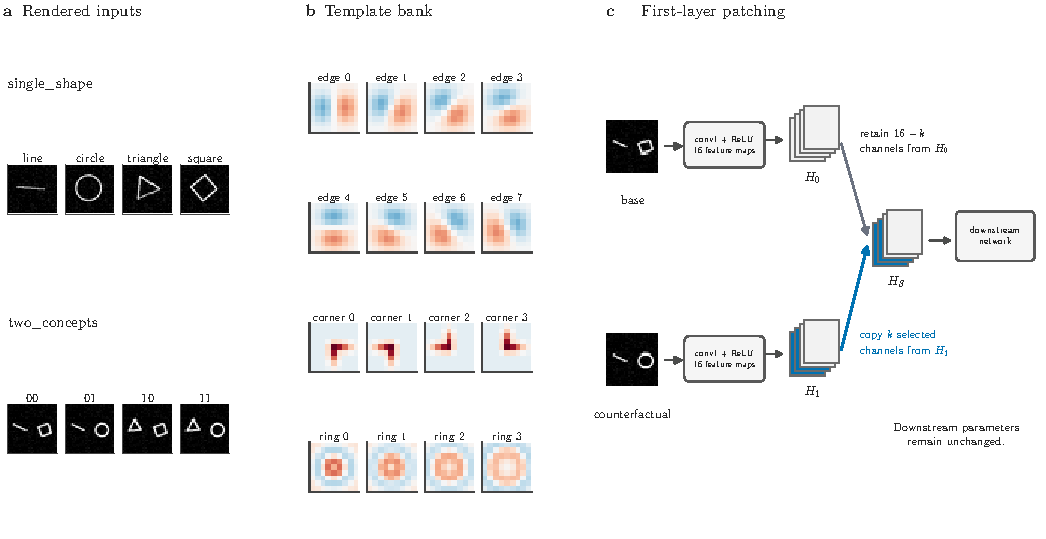
\includegraphics[width=\linewidth]{figures/fig00_overview.pdf}
\caption{Controlled experimental system. \textbf{(a)} Representative inputs from the procedural renderer. \textbf{(b)} The 16 predefined first-layer spatial filters: eight edges, four corners, and four rings. \textbf{(c)} Activation patching replaces a selected set of $k$ post-ReLU first-layer feature maps in a base run with the corresponding maps from a matched counterfactual run, while downstream parameters remain unchanged. Source activations come from in-distribution counterfactual images; the resulting hybrid activation state is nevertheless an intervention and need not itself lie on the model's training manifold.}
\label{fig:overview}
\end{figure}

For learned filter $W_i$ and template $T_j$, structural similarity is
\begin{equation}
\label{eq:template-similarity}
A=\frac{1}{16}\sum_i\max_j\langle \widehat W_i,\widehat T_j\rangle,
\end{equation}
where the inner product is signed cosine similarity after centering and normalizing each filter. A one-to-one matching analysis is retained as a secondary structural check.

\subsection{Retention, release, and matched anchor controls}\label{sec:training}

Template-based models initialize the first convolution from anchor bank $W_{\mathrm{anchor}}$ and optimize
\begin{equation}
\label{eq:training-objective}
\mathcal L=\mathcal L_{\mathrm{CE}}+
\lambda(e)\frac{\lVert W-W_{\mathrm{anchor}}\rVert_F^2}
{\lVert W_{\mathrm{anchor}}\rVert_F^2}.
\end{equation}
The central training comparison uses the same initialization but different regularization schedules. \emph{Retention} keeps $\lambda(e)=1$ for all 200 epochs. \emph{Release} keeps $\lambda=1$ through epoch 10, decays linearly to zero by epoch 80, and remains zero thereafter. Adam uses learning rate $0.003$ and batch size 128, with no learning-rate scheduler or early stopping.

The final fresh-sample specificity experiment replaces the original anchor with three controls while preserving the same retention/release schedules. The primary matched control, \emph{pixel-permuted}, applies one common random permutation of the 81 spatial coordinates to every row of the structured bank. Because the same permutation is applied to all rows, it preserves the complete $16\times16$ Gram matrix, row norms, numerical rank, singular spectrum, and each row's coefficient multiset while destroying the original two-dimensional edge/corner/ring arrangement. Two secondary controls use a generic random rank-10 bank and a generic random full-rank bank. Random anchor realizations are paired across task, architecture, and treatment within block/init replicate.

\subsection{Activation patching, ranking, and output metrics}\label{sec:patching}

For each matched base/counterfactual pair, we cache the post-ReLU first-layer tensor for both images. A patched run starts from the base image and replaces selected feature maps with the corresponding maps from the counterfactual run. No test-set quantity is used to select channels.

The primary selected-channel ranking is the absolute standardized validation-set difference in global-max first-layer activation,
\begin{equation}
\label{eq:channel-ranking}
d_{g,j}=
\frac{\overline z_{g=1,j}-\overline z_{g=0,j}}
{s_j+10^{-6}},
\end{equation}
where $z_j$ is the global maximum of feature map $j$ and $s_j$ is its validation-set standard deviation. The same ranking rule is used for every downstream architecture. Eight same-size random channel orders provide a ranking-independence diagnostic.

Let
\begin{equation}
\label{eq:probability-error}
E_{\mathrm{prob}}(a,b)=
\frac{1}{N}\sum_{i=1}^{N}\lVert p_a^{(i)}-p_b^{(i)}\rVert_2^2
\end{equation}
denote mean squared probability-space error over $N$ matched pairs. The historical patching score is
\begin{equation}
\label{eq:probability-fidelity}
F_{\mathrm{prob}}(S)=
1-\frac{E_{\mathrm{prob}}(S,1)}{E_{\mathrm{prob}}(0,1)}.
\end{equation}
This is a model-normalized counterfactual reconstruction score, not a mediated fraction or a general measure of causal importance.

Because the denominator in \cref{eq:probability-fidelity} varies across models and treatments, later analyses use two primary robustness metrics. Centered logits remove the arbitrary common-logit offset,
\begin{equation}
\label{eq:centered-logits}
\widetilde{\ell}=\ell-\mathrm{mean}(\ell)\mathbf 1,
\end{equation}
and centered-logit fidelity applies the same normalized reconstruction form in that space. The unnormalized probability error reduction is
\begin{equation}
\label{eq:probability-error-reduction}
R_{\mathrm{prob}}(S)=
E_{\mathrm{prob}}(0,1)-E_{\mathrm{prob}}(S,1).
\end{equation}

\subsection{Channel-budget estimand and evidence design}\label{sec:estimand}

For any patching metric $M$, define the within-block release-minus-retention difference at channel count $k$,
\begin{equation}
\label{eq:treatment-difference}
\Delta_b^M(k)=M_b^{\mathrm{release}}(k)-M_b^{\mathrm{retention}}(k),
\end{equation}
and the prespecified small-versus-larger-channel contrast
\begin{equation}
\label{eq:channel-count-contrast}
B_b^M=
\frac{\Delta_b^M(4)+\Delta_b^M(8)}{2}
-\frac{\Delta_b^M(1)+\Delta_b^M(2)}{2}.
\end{equation}
A positive $B$ means only that the release-minus-retention difference is larger on average at $k=4,8$ than at $k=1,2$. It does not imply monotonicity in $k$ or a positive release effect at either larger channel count.

Matched image pairs are repeated measurements within a model/block and are never treated as independent inferential replicates. The principal evidence comes from three fresh-sample designs. First, a prospectively frozen channel-budget test uses 20 new \texttt{two\_concepts} renderer blocks in the TinyCNN setting. Second, a prospectively frozen architecture study uses 100 new blocks, four paired initialization replicates, two tasks, two treatments, and 16 downstream CNN variants; the four init replicates are averaged within block before inference. Third, the matched-anchor specificity study uses 100 further fresh blocks, four init/anchor replicates, two tasks, four diagnostic architectures, four anchor families, and two treatments, again averaging the four replicates within block. The latter two designs each train 25,600 models but have inferential sample size $n=100$, not 25,600.

Alternative-metric reanalysis of saved prospective checkpoints and the later Greenhouse--Geisser, permutation, Friedman, and random-channel architecture diagnostics are explicitly post hoc with respect to the original results, although their analysis definitions were frozen before recomputation. Complete developmental and secondary schedule analyses are retained in the appendix but are not pooled with fresh-sample tests.

\section{Results}\label{sec:results}

\subsection{Structural retention does not determine the patching signature}\label{sec:structural}

Retention produces the intended weight-space effect. In the larger schedule/task sensitivity sample, \texttt{two\_concepts}/TinyCNN models under constant regularization have mean template similarity 0.944 versus 0.574 under release, while mean test accuracy is 98.05\% versus 99.45\%. In the corresponding two-layer model, similarities are 0.999 and 0.896 while accuracies are 99.11\% and 99.26\%. One-to-one matching gives the same structural conclusion and rules out the trivial explanation that many learned filters merely match the same few templates (\Cref{app:kernel-matching}).

\Cref{fig:kernel-gallery} provides a representative visualization. It is deliberately treated as structural evidence only: neither visual resemblance nor the score in \cref{eq:template-similarity} establishes semantic purity or functional influence.

\begin{figure}[t]
\centering
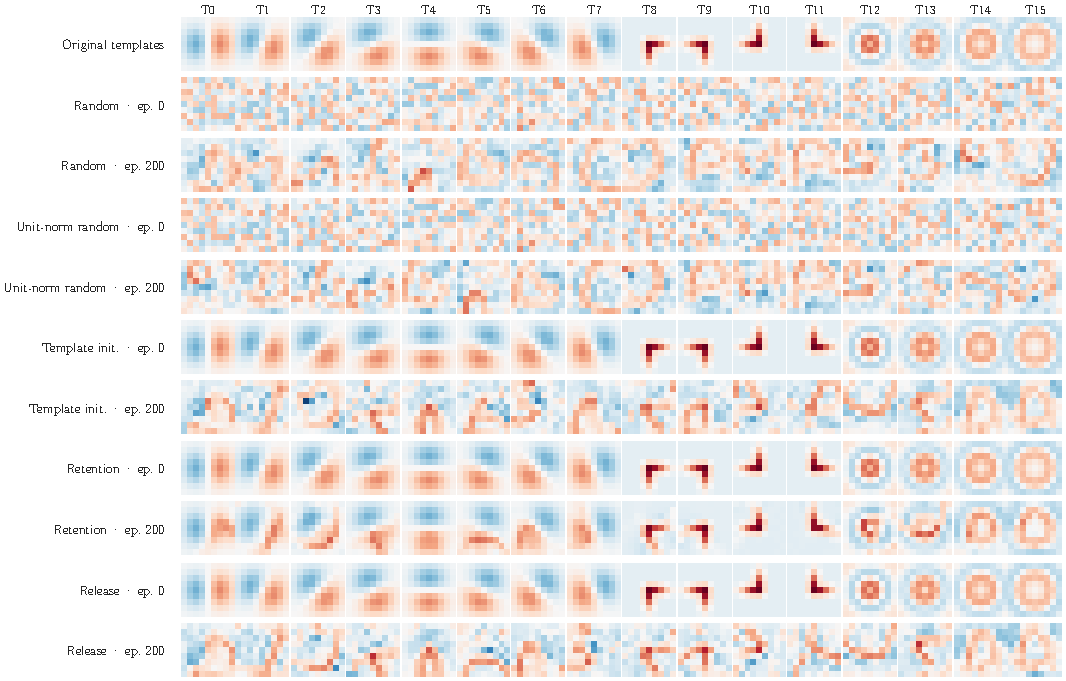
\includegraphics[width=\linewidth]{figures/fig05_kernel_gallery.pdf}
\caption{Representative first-layer kernels from a \texttt{two\_concepts}/TinyCNN checkpoint. The top row shows the predefined bank; later rows show saved filters under the developmental training conditions, reordered by one-to-one template matching for display. Retention preserves visibly template-like kernels, whereas released filters move farther from the bank. The inferential claims in the paper use replicate-level structural and intervention statistics rather than this example.}
\label{fig:kernel-gallery}
\end{figure}

The functional comparison is not fixed by that structural separation. In the prospectively frozen 20-block TinyCNN test, the historical probability-fidelity contrast is
\begin{equation}
\label{eq:prospective-channel-result}
\bar B_{\mathrm{prob}}=0.33098,
\qquad
95\%\ \mathrm{CI}=[0.27368,0.38827],
\end{equation}
with $t_{19}=12.09$, $p=2.28\times10^{-10}$, and all 20 block-level values positive. The pointwise release-minus-retention differences are $-0.3459$, $-0.3317$, $-0.0221$, and $+0.0065$ at $k=1,2,4,8$, respectively. Thus a single patch budget would describe only one slice of the treatment comparison.

\subsection{The channel-budget contrast survives alternative metrics, not identical curves}\label{sec:metric-robustness}

The original probability fidelity has a model-specific denominator, and the frozen metric reanalysis confirms that this denominator changes substantially between retention and release. The probability-space base-to-counterfactual error scale differs by $+0.8486$ on average in the prospective TinyCNN setting, and the centered-logit scale differs by $+126.54$. The original normalization is therefore not innocuous.

Nevertheless, the prespecified contrast in \cref{eq:channel-count-contrast} remains positive under both frozen alternatives. Centered-logit fidelity gives $B=+0.17888$ (95\% CI $[+0.12727,+0.23049]$, Holm $p=6.95\times10^{-7}$), while probability error reduction gives $B=+0.89441$ (95\% CI $[+0.78630,+1.00252]$, Holm $p=8.59\times10^{-13}$).

Panel~(a) of \cref{fig:main-results} is important for the interpretation: the alternative metrics support the same \emph{sign of the prespecified $B$ contrast}, but not the same pointwise treatment curve. In particular, unnormalized probability error reduction becomes strongly positive at $k=4,8$, whereas the historical normalized probability score is close to zero there. We therefore treat metric agreement at the level of the frozen estimand as robustness, not as evidence that the metrics are interchangeable.

\begin{figure}[t]
\centering
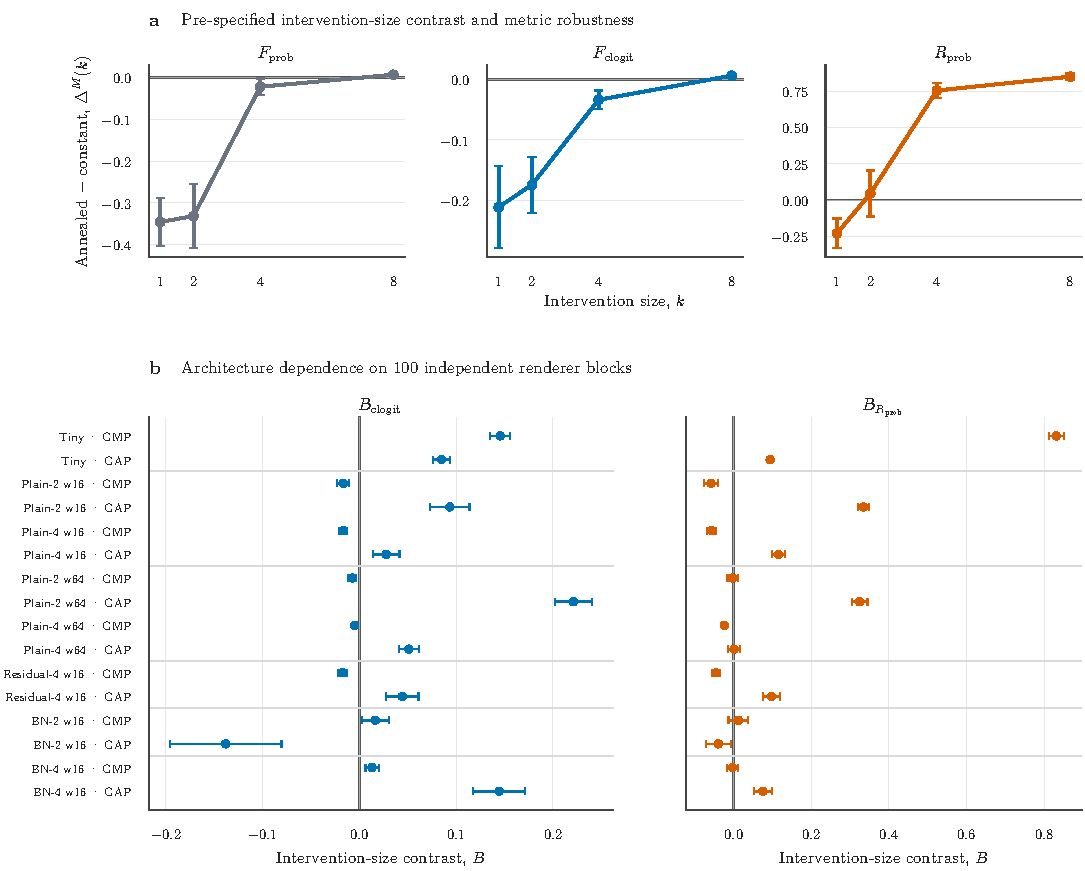
\includegraphics[width=\linewidth]{figures/fig06_main_results.pdf}
\caption{Channel-budget and architecture robustness. \textbf{(a)} Release-minus-retention treatment differences $\Delta^M(k)$ in the prospective \texttt{two\_concepts}/TinyCNN experiment under the historical normalized probability score, centered-logit fidelity, and unnormalized probability error reduction. The three metrics agree on a positive small-versus-larger-channel contrast $B$ but not on the detailed pointwise curve. \textbf{(b)} Architecture-specific $B$ on the primary \texttt{two\_concepts} task for 16 prospectively frozen downstream architectures. Each point averages four initialization replicates within each of 100 fresh renderer blocks; bars are marginal 95\% $t$ intervals. The two primary metrics are shown separately because their numerical scales are not comparable.}
\label{fig:main-results}
\end{figure}

\subsection{Downstream architecture is a major conditioning variable}\label{sec:architecture}

Holding the first-layer intervention tensor, training comparison, validation ranking, counterfactual construction, and primary metrics fixed, the 16-architecture fresh-sample study finds strong heterogeneity:
\begin{equation}
\label{eq:architecture-omnibus-clogit}
F_{15,1485}=77.09,\quad \eta_p^2=0.438
\end{equation}
for centered-logit fidelity and
\begin{equation}
\label{eq:architecture-omnibus-prob}
F_{15,1485}=656.70,\quad \eta_p^2=0.869
\end{equation}
for probability error reduction. The fresh TinyGMP-minus-Plain2-GMP bridge is $+0.16226$ (95\% CI $[+0.14970,+0.17481]$) for centered logits and $+0.88960$ (95\% CI $[+0.86212,+0.91707]$) for probability error reduction.

The pattern in panel~(b) of \cref{fig:main-results} is not a single monotone effect of depth or pooling. Under GMP, most of the Tiny-to-plain shift occurs when the first downstream convolution is added; adding further plain depth changes little. Under GAP, the depth pattern differs. GAP-versus-GMP contrasts are large but reverse direction across backbones. Residual-versus-plain depth-4 contrasts are comparatively small, while BatchNorm effects depend on depth, pooling, and metric. The defensible conclusion is therefore architecture dependence, not a universal law about any single architectural component.

A frozen post hoc diagnostic analysis addresses two reviewer-sensitive alternatives. First, the architecture omnibus survives Greenhouse--Geisser correction, 100,000 within-block permutations, and Friedman rank tests; the Holm-adjusted permutation $p$ value is $2.0\times10^{-5}$ for both primary metrics. Second, architecture heterogeneity remains when $B$ is computed from the mean over eight random channel orders, again with Holm permutation $p=2.0\times10^{-5}$ for both metrics. The architecture result is therefore not solely produced by the validation-derived channel ranking. Ranking still matters quantitatively: selected-versus-random architecture-mean Spearman correlation is $0.256$ for centered logits and $0.724$ for probability error reduction (\Cref{app:architecture-posthoc}).

\subsection{The original two-dimensional template structure has a conditional functional effect}\label{sec:anchor-specificity}

The strongest remaining alternative after the architecture study was that retention/release effects might arise for any anchor, with the edge/corner/ring structure playing no special role. The fresh matched-anchor experiment addresses this directly. Its primary control applies the same random permutation of spatial coordinates to every template, preserving the full Gram matrix, numerical rank, singular spectrum, row norms, and row coefficient multisets while destroying the original two-dimensional arrangement.

Averaged over the four diagnostic architectures on \texttt{two\_concepts}, selected-channel centered-logit $B$ differs between structured and pixel-permuted anchors by $+0.05743$ (95\% CI $[+0.05116,+0.06369]$, Holm sign-flip $p=2.0\times10^{-5}$). The 90\% interval $[+0.05219,+0.06266]$ lies entirely outside the frozen equivalence margin $\pm0.01704$, so this effect is both statistically distinguishable from zero and not practically equivalent under the prespecified rule.

For probability error reduction, the mean difference is $+0.04563$ (95\% CI $[+0.03728,+0.05397]$, Holm sign-flip $p=2.0\times10^{-5}$). Here the 90\% interval $[+0.03864,+0.05261]$ lies inside the wider frozen equivalence margin $\pm0.06594$; the difference is therefore precisely nonzero but practically equivalent by the prespecified smallest effect size of interest. Both statements are required for an accurate summary.

The average also hides a strong architecture interaction. The structured-minus-pixel-permuted selected-channel effect is positive for \texttt{tiny\_gmp}, \texttt{tiny\_gap}, and \texttt{plain2\_w16\_gap}, but negative for \texttt{plain2\_w16\_gmp} under both primary metrics. The interaction has partial $\eta^2=0.481$ for centered logits and $0.614$ for probability error reduction, with Holm permutation $p=2.0\times10^{-5}$ for both. Panel~(a) of \cref{fig:anchor-specificity} shows the sign reversal directly.

\begin{figure}[t]
\centering
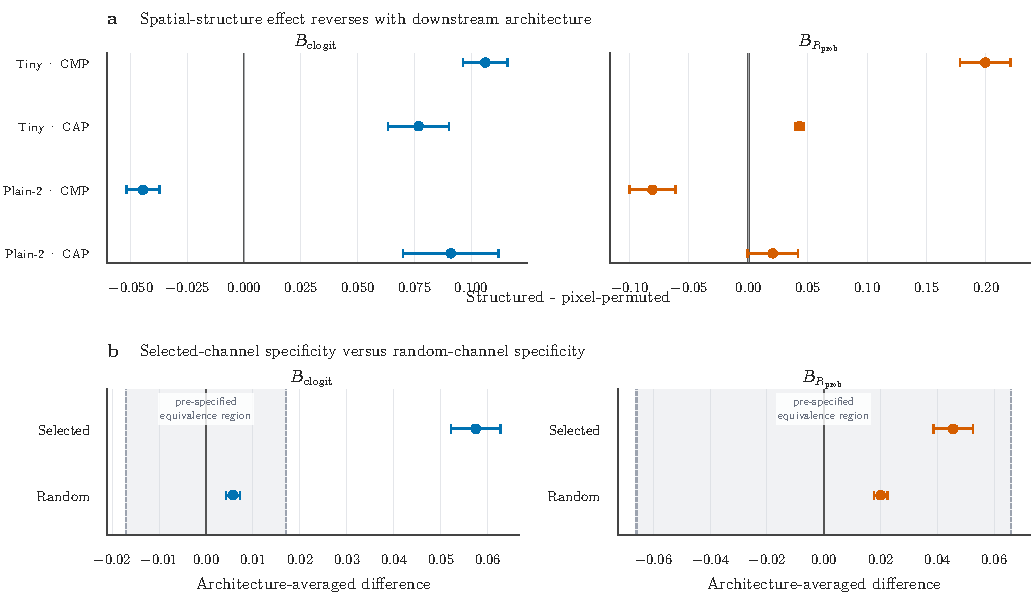
\includegraphics[width=\linewidth]{figures/fig07_anchor_specificity.pdf}
\caption{Fresh matched-anchor specificity experiment. \textbf{(a)} Architecture-specific selected-channel difference in $B$ between the original structured bank and its common pixel-permuted control on \texttt{two\_concepts}. The spatial effect reverses sign in \texttt{plain2\_w16\_gmp}. Bars are paired 95\% $t$ intervals over 100 fresh renderer blocks. \textbf{(b)} Architecture-averaged structured-minus-pixel-permuted effects for validation-selected and random channel sets. Bars are 90\% intervals used by the frozen TOST procedure; shaded regions denote the prespecified equivalence margins. Selected-channel centered-logit specificity is not equivalent, whereas the probability-error average and both random-channel effects are practically equivalent under their frozen margins.}
\label{fig:anchor-specificity}
\end{figure}

The random-channel diagnostic constrains the interpretation further. Averaged across architectures, structured-minus-pixel-permuted random-channel $B$ is only $+0.00571$ for centered logits and $+0.02007$ for probability error reduction. Both are statistically distinguishable from zero but practically equivalent under the same frozen margins. The spatial-prior effect is therefore much more concentrated in the validation-selected channel analysis than in arbitrary same-size channel subsets.

Finally, the secondary anchor controls argue against numerical rank as the main explanation. On the primary task, pixel-permuted and generic random rank-10 anchors are generally similar, and random rank-10 versus random full-rank differences are generally small after the frozen family corrections. The original two-dimensional organization is the anchor property most clearly isolated by the selected-channel result, but its sign and practical magnitude remain architecture- and metric-dependent.

\subsection{Integrity and secondary evidence}\label{sec:secondary}

The fresh anchor experiment completes all 25,600 planned training jobs and evaluations. Maximum full-patch and no-op logit identity errors are zero, and the maximum structured-versus-pixel-permuted Gram-matrix discrepancy is $6.66\times10^{-16}$. The earlier independent checkpoint audit also reproduces central developmental metrics at 32 fixed checkpoints within prespecified numerical tolerances. Secondary schedule, task, ranking, and energy-matched analyses are reported in the appendix; they motivate and delimit the main estimands but are not treated as independent repetitions of the fresh-sample tests.

\section{Discussion}\label{sec:discussion}

The results separate weight-space structure from intervention-based function in a way that neither literature alone makes explicit. Work on predefined, fixed, and Gabor-based filters shows that spatial structure can be useful, robust, or even unnecessary for predictive performance depending on how later layers recombine it \citep{linse_2024_predefined-filters,gaudio_2023_fixed-filters,gavrikov_2023_random-convolutions,molaei_2020_gabor-filter-structure}. Our retention condition confirms that such structure can be maintained almost exactly. But high structural similarity does not determine a unique patching signature. The same first-layer retention/release comparison changes with channel budget, and the same first-layer intervention propagates differently through different downstream architectures.

The matched-anchor experiment sharpens that conclusion. The original spatial arrangement is not merely decorative: under centered-logit fidelity, selected-channel $B$ differs clearly from a control that preserves the bank's complete non-spatial channel geometry. At the same time, this is not a universal template benefit. The effect reverses in one architecture, is practically small under the probability-error smallest effect size of interest when averaged across architectures, and is much smaller for random channel sets. The most defensible interpretation is therefore that designed spatial structure changes where the release-versus-retention functional difference concentrates, conditional on the downstream computation and on how channels are selected.

This distinction parallels a broader lesson from concept-based and mechanistic interpretability. Alignment, decodability, and causal influence answer different questions \citep{margeloiu_2021_concept-bottleneck-alignment,nicolson_2025_explaining-explainability,sharma_2026_encoding-without-influence}. Likewise, activation patching is a family of interventions whose conclusions depend on intervention and evaluation choices \citep{heimersheim_2024_activation-patching,zhang_2024_activation-patching,miller_2024_circuit-faithfulness}. Our contribution is to show this conditionality in a controlled vision setting where the internal representation is deliberately structured and the input counterfactuals are exact. Channel budget, downstream architecture, output metric, spatial anchor structure, and ranking rule are not interchangeable implementation details; they define materially different measurements.

The practical implication is methodological rather than prescriptive. A patching result should be reported together with the number and type of components patched, the output metric, the architecture through which the intervention propagates, the channel-selection rule, and the source of replacement activations. Weight-space similarity should be reported separately from functional intervention effects. When a null comparison is scientifically meaningful, equivalence should be tested rather than inferred from nonsignificance. These practices do not make patching a complete mechanistic explanation, but they make the claim being tested substantially clearer.

\section{Limitations}\label{sec:limitations}

\begin{itemize}
\item The experiments use two related synthetic image tasks, one family of first-layer spatial templates, and small CNNs. Exact counterfactual control is a strength for measurement, but the results do not establish natural-image, large-CNN, vision-transformer, or language-model generalization.
\item Patching replaces complete post-ReLU feature maps with activations from an in-distribution matched counterfactual. The source activations are therefore not generated by artificial input corruption, but the hybrid activation state can still be off-manifold for the trained model.
\item The validation ranking uses global-max first-layer activation for every architecture, including GAP variants. This keeps ranking fixed while architecture changes, but it may favor some representations. Random-channel diagnostics show that architecture dependence survives without that ranking, while the fresh specificity experiment shows that the structure-specific effect is much smaller for random channels.
\item The historical normalized probability score has a model-specific denominator that differs across treatments. Later analyses therefore use centered-logit and unnormalized probability metrics. Agreement is strongest at the level of the prespecified $B$ contrast and architecture omnibus; detailed pointwise curves and practical-effect conclusions can differ across metrics.
\item The anchor-specificity probability-error difference is statistically nonzero but practically equivalent under the frozen margin. It should not be described as a practically important average effect merely because its $p$ value is small.
\item The architecture-factor decompositions and the later Greenhouse--Geisser, Friedman, structural-versus-functional, and random-channel diagnostics are controlled or frozen analyses but some are post hoc with respect to the original architecture outcomes. They delimit the result; they do not provide independent prospective confirmation.
\item Filter-template similarity is a geometric weight-space score. Neither that score nor the visual appearance of filters establishes human interpretability, semantic purity, a unique mechanism, or an identifiable causal abstraction \citep{meloux_2025_mechanistic-identifiability,sutter_2025_causal-abstraction-limits}.
\end{itemize}

\section{Conclusion}\label{sec:conclusion}

Preserving a predefined first-layer spatial basis does not yield a single activation-patching signature. In controlled CNNs with exact matched counterfactuals, the release-versus-retention comparison changes with the number of patched channels and varies strongly across downstream architectures. Those conclusions survive alternative output metrics and sphericity-robust, permutation-based, and random-channel diagnostics. A fresh matched-anchor experiment further shows that the original two-dimensional edge/corner/ring arrangement itself changes selected-channel patch-budget behavior beyond the bank's Gram matrix, rank, and singular spectrum---but the effect is architecture-dependent, metric-dependent, and much smaller for random channel sets. Structural retention, selected-channel functional concentration, and intervention-based measurement should therefore be treated as distinct empirical quantities.

\section{Data and code availability}\label{sec:availability}

The experiments use procedurally rendered synthetic images. The research artifact contains the renderer, model and anchor definitions, training and evaluation code, frozen protocols, execution manifests, complete paper-facing result tables, analysis scripts, matched-anchor integrity checks, and the independent checkpoint audit. Large raw checkpoints and per-model evaluator outputs are retained outside the manuscript-facing archive, while all aggregate data needed to reproduce the reported paper statistics and figures are versioned. For anonymous review, the manuscript does not link the current working repository because it identifies the authors. An anonymized archival artifact and DOI will be prepared if required by the venue.

\bibliography{../literature/references.bib}

\clearpage
\appendix
\noindent\textbf{Appendix organization.} \Cref{app:specificity} reports the fresh matched-anchor specificity experiment and the post hoc architecture diagnostics. \Cref{app:final-robustness} gives the complete metric- and architecture-robustness summaries. \Cref{app:confirmation} reports the prospective channel-budget and schedule/task sensitivity analyses. \Cref{app:historical} preserves the developmental analyses that motivated the prospective estimand. \Cref{app:kernel-matching} reports the complete filter-matching table.

\section{Matched-anchor specificity and architecture diagnostics}\label{app:specificity}

This appendix reports the complete paper-facing statistics for the fresh anchor-specificity experiment and the frozen post hoc architecture diagnostics. The anchor-specificity experiment is prospectively frozen fresh-sample evidence; the architecture diagnostics are outcome-informed post hoc robustness analyses and are labeled accordingly.

\subsection{Fresh matched-anchor specificity experiment}\label{app:anchor-specificity}

The fresh experiment uses 100 renderer blocks, four init/anchor replicates per block, two tasks, four diagnostic downstream architectures, four anchor families, and two regularization schedules, for 25,600 trained and evaluated models. The inferential unit is the renderer block after averaging the four init/anchor replicates.

The primary comparison is the original structured edge/corner/ring bank against a bank formed by applying one common random permutation of the 81 spatial coordinates to every template row. This pixel-permuted control preserves, to numerical tolerance, every row norm, the complete $16\times16$ Gram matrix, numerical rank, singular spectrum, and row coefficient multisets while destroying the original 2D spatial arrangement.

\begin{table}[h]
\caption{Primary selected-channel structured-minus-pixel-permuted channel-count contrast on \texttt{two\_concepts}. Difference tests use 100,000 sign-flip permutations and Holm correction across the two primary metrics. Equivalence uses the frozen TOST margins and 90\% confidence intervals.}
\label{tab:anchor-primary}
\centering
\footnotesize
\setlength{\tabcolsep}{3pt}
\begin{tabular}{lrrrr}
\toprule
Metric & Mean difference & 95\% CI & Holm diff. $p$ & Equivalence result \\
\midrule
Centered-logit fidelity & +0.05743 & [0.05116, 0.06369] & $2.0\times10^{-5}$ & not equivalent ($\delta=0.01704$) \\
Probability error reduction & +0.04563 & [0.03728, 0.05397] & $2.0\times10^{-5}$ & equivalent ($\delta=0.06594$) \\
\bottomrule
\end{tabular}
\end{table}

For centered logits, the 90\% interval is $[0.05219,0.06266]$ and the Holm-adjusted TOST $p$ value is 1. For probability error reduction, the 90\% interval is $[0.03864,0.05261]$ and the Holm-adjusted TOST $p$ value is $5.03\times10^{-6}$. Thus a statistically nonzero probability-error difference is nevertheless practically equivalent under the prespecified smallest effect size of interest.

\subsection{Architecture dependence of spatial specificity}\label{app:anchor-architecture}

The structured-minus-pixel-permuted effect varies strongly across the four prospectively frozen diagnostic architectures.

\begin{table}[h]
\caption{Architecture-specific selected-channel structured-minus-pixel-permuted $B$ differences on \texttt{two\_concepts}. Intervals are paired 95\% $t$ intervals over 100 renderer blocks.}
\label{tab:anchor-architectures}
\centering
\small
\begin{tabular}{lrr}
\toprule
Architecture & Centered-logit difference & Probability-error difference \\
\midrule
\texttt{tiny\_gmp} & +0.10624 & +0.19953 \\
\texttt{tiny\_gap} & +0.07690 & +0.04308 \\
\texttt{plain2\_w16\_gmp} & -0.04453 & -0.08067 \\
\texttt{plain2\_w16\_gap} & +0.09109 & +0.02057 \\
\bottomrule
\end{tabular}
\end{table}

The corresponding within-block architecture interaction is
$F(3,297)=91.79$, partial $\eta^2=0.481$, Holm permutation $p=2.0\times10^{-5}$ for centered-logit fidelity, and
$F(3,297)=157.70$, partial $\eta^2=0.614$, Holm permutation $p=2.0\times10^{-5}$ for probability error reduction. The sign reversal in \texttt{plain2\_w16\_gmp} rules out a universal positive effect of the original spatial arrangement.

\subsection{Random-channel specificity diagnostic}\label{app:anchor-random}

Repeating the primary comparison after averaging over eight random channel orders produces much smaller spatial-structure effects.

\begin{table}[h]
\caption{Architecture-averaged structured-minus-pixel-permuted $B$ for random channel sets on \texttt{two\_concepts}. Both effects are statistically distinguishable from zero but practically equivalent under the frozen margins.}
\label{tab:anchor-random}
\centering
\small
\begin{tabular}{lrr}
\toprule
Metric & Mean difference & 95\% CI \\
\midrule
Centered-logit fidelity & +0.00571 & [0.00392, 0.00750] \\
Probability error reduction & +0.02007 & [0.01722, 0.02291] \\
\bottomrule
\end{tabular}
\end{table}

The random-channel spatial-structure interaction remains detectable but is smaller for centered logits: partial $\eta^2=0.0683$ with permutation $p=8.0\times10^{-5}$. For probability error reduction it remains substantial, partial $\eta^2=0.2910$ with permutation $p=1.0\times10^{-5}$. These are prespecified robustness diagnostics, not a second primary family.

Secondary anchor contrasts show that pixel-permuted and generic random rank-10 anchors are generally similar on the primary task, and that random rank-10 and random full-rank anchors are also generally similar after the frozen family corrections. The original 2D arrangement, rather than numerical rank alone, is therefore the anchor property most clearly distinguished by the selected-channel analysis.

Integrity checks pass exactly for the intervention identities: maximum full-patch and no-op logit errors are zero. The maximum structured-versus-pixel-permuted Gram-matrix discrepancy is $6.66\times10^{-16}$.

\subsection{Post hoc architecture robustness diagnostics}\label{app:architecture-posthoc}

The original 16-architecture result was prospectively frozen. After seeing that result, a separate frozen diagnostic analysis tested whether its omnibus conclusion depended on the uncorrected sphericity assumption or on the validation-derived channel ranking. These analyses are explicitly post hoc.

\begin{table}[h]
\caption{Sphericity-robust and permutation-based architecture omnibus diagnostics on the primary \texttt{two\_concepts} task. Permutation $p$ values use 100,000 within-block permutations and are Holm adjusted across the two metrics within each analysis kind.}
\label{tab:architecture-posthoc}
\centering
\footnotesize
\setlength{\tabcolsep}{3pt}
\begin{tabular}{lrrrr}
\toprule
Metric & GG $\epsilon$ & GG $p$ & Permutation Holm $p$ & Friedman $p$ \\
\midrule
Centered-logit fidelity & 0.1861 & $1.56\times10^{-34}$ & $2.0\times10^{-5}$ & $3.52\times10^{-146}$ \\
Probability error reduction & 0.5973 & $<10^{-300}$ & $2.0\times10^{-5}$ & $7.79\times10^{-200}$ \\
\bottomrule
\end{tabular}
\end{table}

Architecture heterogeneity also remains when $B$ is computed from the mean over eight random channel orders: Holm-adjusted permutation $p=2.0\times10^{-5}$ for both primary metrics. The selected-versus-random architecture-mean Spearman correlation is $0.256$ for centered logits and $0.724$ for probability error reduction.

For the historical TinyGMP-minus-Plain2-GMP bridge using random channel sets, the mean difference is $+0.002765$ (95\% CI $[+0.000014,+0.005515]$, Holm $p=0.0488$) for centered logits and $+0.319871$ (95\% CI $[+0.312788,+0.326953]$, Holm $p=2.76\times10^{-96}$) for probability error reduction. The architecture conclusion is therefore not solely a consequence of the selected-channel ranking, although ranking materially changes effect magnitude and architecture ordering.

\clearpage
\section{Final metric and architecture robustness analyses}\label{app:final-robustness}

This appendix gives the complete paper-facing summaries for the two robustness analyses added after the initial prospective/sensitivity manuscript: the frozen metric-sensitivity reanalysis and the prospectively frozen architecture study. Machine-readable block-level values, design manifests, integrity checks, and the full control diagnostics are versioned under \texttt{analysis/metric\_sensitivity\_001/} and \texttt{analysis/architecture\_robustness\_001/}. The main text reports only the estimates needed for the central argument.

\subsection{Frozen metric-sensitivity analysis}\label{app:metric-sensitivity}

The metric-sensitivity analysis reuses saved checkpoints from the prospective channel-count and schedule/task sensitivity experiments. It was designed after the historical probability-fidelity results were known, so it is post hoc with respect to those original results; however, the alternative metric definitions and analysis plan were frozen before their values were computed. No model was retrained and the original validation-derived channel rankings were reused.

For the primary prospective \texttt{two\_concepts}/TinyCNN/activation-contrast setting, \Cref{tab:app-metric-pointwise} gives the full pointwise annealed-minus-constant curves under the two alternative primary metrics.

\begin{table}[h]
\caption{Prospective TinyCNN pointwise treatment contrasts under the frozen alternative metrics.}
\label{tab:app-metric-pointwise}
\centering
\small
\begin{tabular}{lrrr}
\toprule
Metric & $k$ & Mean $\Delta$ & 95\% CI \\
\midrule
Centered-logit fidelity & 1 & -0.21134 & [-0.27899, -0.14369] \\
Centered-logit fidelity & 2 & -0.17452 & [-0.22078, -0.12825] \\
Centered-logit fidelity & 4 & -0.03405 & [-0.04939, -0.01871] \\
Centered-logit fidelity & 8 & +0.00595 & [+0.00253, +0.00937] \\
\addlinespace[2pt]
Probability error reduction & 1 & -0.22942 & [-0.33033, -0.12852] \\
Probability error reduction & 2 & +0.04493 & [-0.11443, +0.20428] \\
Probability error reduction & 4 & +0.75429 & [+0.70327, +0.80530] \\
Probability error reduction & 8 & +0.85004 & [+0.82915, +0.87093] \\
\bottomrule
\end{tabular}
\end{table}

The corresponding $B$ contrasts are $+0.178881$ (95\% CI $[+0.127268,+0.230494]$) for centered-logit fidelity and $+0.894411$ (95\% CI $[+0.786301,+1.002522]$) for probability error reduction. Holm-adjusted $p$ values for the two-metric family are $6.95\times10^{-7}$ and $8.59\times10^{-13}$, respectively.

The release-minus-retention base-to-counterfactual error scales are themselves different. In TinyCNN the probability input-effect-scale contrast is $+0.848558$ (95\% CI $[+0.826701,+0.870416]$), and the centered-logit input-effect-scale contrast is $+126.537$ (95\% CI $[+120.845,+132.229]$). In TwoLayerCNN the corresponding contrasts are $+0.062062$ and $+211.368$. Thus the historical normalized metric cannot be treated as though its denominator were constant across treatments.

The same frozen analysis applied to the schedule/task sensitivity experiment gives the default-release results in \Cref{tab:app-metric-sensitivity}.

\begin{table}[h]
\caption{Schedule/task sensitivity default-release $B$ contrasts under the frozen alternative metrics. Values are release minus constant $\lambda=1$ under the original activation-contrast ranking.}
\label{tab:app-metric-sensitivity}
\centering
\small
\begin{tabular}{llrr}
\toprule
Task & Architecture & $B_{\mathrm{clogit}}$ & $B_{R_{\mathrm{prob}}}$ \\
\midrule
single shape & TinyCNN & +0.05660 & +0.33747 \\
single shape & TwoLayerCNN & +0.05700 & -0.01622 \\
two concepts & TinyCNN & +0.13427 & +0.80239 \\
two concepts & TwoLayerCNN & -0.01953 & -0.05497 \\
\bottomrule
\end{tabular}
\end{table}

The maximum absolute discrepancy between recomputed and stored historical probability fidelity is $1.24\times10^{-7}$. Maximum full-patch and no-op logit identity errors are zero.

\subsection{Primary architecture robustness analyses}\label{app:architecture-primary}

The architecture robustness experiment uses 100 fresh renderer blocks, four paired initialization replicates per block, 16 downstream architectures, two tasks, and the two central treatments. Initialization replicates are averaged before inference. The primary task is \texttt{two\_concepts}; the inferential unit is therefore the renderer block ($n=100$) for each architecture-level comparison.

\begin{table}[h]
\caption{Frozen repeated-measures architecture omnibus tests on \texttt{two\_concepts}.}
\label{tab:app-architecture-omnibus}
\centering
\small
\begin{tabular}{lrrrr}
\toprule
Metric & $F$ & df & partial $\eta^2$ & Holm $p$ \\
\midrule
centered\_logit\_fidelity & 77.09 & 15, 1485 & 0.438 & $2.40\times10^{-173}$ \\
prob\_error\_reduction & 656.70 & 15, 1485 & 0.869 & 0 (machine precision) \\
\bottomrule
\end{tabular}
\end{table}

For probability error reduction, the computed upper-tail $p$ value is numerically zero at double precision; this is reported as a machine-precision underflow rather than a literal probability of zero.

\begin{table}[h]
\caption{Frozen fresh-sample architecture bridge contrast, \texttt{tiny\_gmp} minus \texttt{plain2\_w16\_gmp}.}
\label{tab:app-architecture-bridge}
\centering
\small
\begin{tabular}{lrrr}
\toprule
Metric & Mean difference in $B$ & 95\% CI & Holm $p$ \\
\midrule
centered\_logit\_fidelity & +0.16226 & [+0.14970, +0.17481] & $1.66\times10^{-45}$ \\
prob\_error\_reduction & +0.88960 & [+0.86212, +0.91707] & $3.24\times10^{-82}$ \\
\bottomrule
\end{tabular}
\end{table}

\subsection{Architecture-specific estimates}\label{app:architecture-estimates}

\Cref{tab:app-architecture-estimates} reports every architecture mean and marginal 95\% $t$ interval for the two frozen primary metrics.

{\scriptsize
\setlength{\tabcolsep}{3pt}
\begin{longtable}{lrrrr}
\caption{\texttt{two\_concepts} architecture means for $B$.}\label{tab:app-architecture-estimates}\\
\toprule
Architecture & $B_{\mathrm{clogit}}$ & 95\% CI & $B_{R_{\mathrm{prob}}}$ & 95\% CI \\
\midrule
\endfirsthead
\toprule
Architecture & $B_{\mathrm{clogit}}$ & 95\% CI & $B_{R_{\mathrm{prob}}}$ & 95\% CI \\
\midrule
\endhead
\bottomrule
\endfoot
tiny\_gmp & +0.1456 & [+0.1352, +0.1560] & +0.8315 & [+0.8122, +0.8508] \\
tiny\_gap & +0.0849 & [+0.0764, +0.0934] & +0.0944 & [+0.0901, +0.0986] \\
plain2\_w16\_gmp & -0.0167 & [-0.0227, -0.0106] & -0.0581 & [-0.0757, -0.0404] \\
plain2\_w16\_gap & +0.0936 & [+0.0734, +0.1139] & +0.3348 & [+0.3207, +0.3488] \\
plain4\_w16\_gmp & -0.0168 & [-0.0211, -0.0124] & -0.0561 & [-0.0675, -0.0447] \\
plain4\_w16\_gap & +0.0277 & [+0.0138, +0.0416] & +0.1160 & [+0.0992, +0.1328] \\
plain2\_w64\_gmp & -0.0072 & [-0.0113, -0.0031] & -0.0021 & [-0.0152, +0.0111] \\
plain2\_w64\_gap & +0.2213 & [+0.2022, +0.2404] & +0.3247 & [+0.3045, +0.3449] \\
plain4\_w64\_gmp & -0.0049 & [-0.0068, -0.0029] & -0.0238 & [-0.0282, -0.0194] \\
plain4\_w64\_gap & +0.0511 & [+0.0408, +0.0614] & +0.0013 & [-0.0150, +0.0176] \\
res4\_w16\_gmp & -0.0175 & [-0.0216, -0.0133] & -0.0448 & [-0.0554, -0.0342] \\
res4\_w16\_gap & +0.0444 & [+0.0276, +0.0611] & +0.0974 & [+0.0756, +0.1192] \\
bn2\_w16\_gmp & +0.0165 & [+0.0024, +0.0306] & +0.0127 & [-0.0128, +0.0382] \\
bn2\_w16\_gap & -0.1382 & [-0.1960, -0.0804] & -0.0390 & [-0.0706, -0.0074] \\
bn4\_w16\_gmp & +0.0132 & [+0.0063, +0.0201] & -0.0023 & [-0.0163, +0.0116] \\
bn4\_w16\_gap & +0.1445 & [+0.1177, +0.1713] & +0.0757 & [+0.0532, +0.0983] \\
\end{longtable}
\normalsize
}

\subsection{Prespecified architecture-factor contrasts}\label{app:architecture-factors}

\Cref{tab:app-architecture-factors} gives all prespecified factor contrasts on the primary \texttt{two\_concepts} task. Holm adjustment is applied within metric, task, and factor family exactly as frozen in the architecture robustness protocol. The signs are alternative architecture minus reference architecture as named in each row.

\begin{landscape}
{\scriptsize
\setlength{\tabcolsep}{3pt}
\begin{longtable}{p{.10\linewidth}p{.38\linewidth}rrrr}
\caption{Architecture-factor contrasts.}\label{tab:app-architecture-factors}\\
\toprule
Family & Contrast & $\Delta B_{\mathrm{clogit}}$ & Holm $p$ & $\Delta B_{R_{\mathrm{prob}}}$ & Holm $p$ \\
\midrule
\endfirsthead
\toprule
Family & Contrast & $\Delta B_{\mathrm{clogit}}$ & Holm $p$ & $\Delta B_{R_{\mathrm{prob}}}$ & Holm $p$ \\
\midrule
\endhead
\bottomrule
\endfoot
pooling & tiny: GAP - GMP & -0.0607 & $7.25\times10^{-14}$ & -0.7372 & $4.41\times10^{-88}$ \\
pooling & plain2\_w16: GAP - GMP & +0.1103 & $3.42\times10^{-17}$ & +0.3929 & $3.70\times10^{-56}$ \\
pooling & plain4\_w16: GAP - GMP & +0.0445 & $7.53\times10^{-8}$ & +0.1721 & $4.57\times10^{-28}$ \\
pooling & plain2\_w64: GAP - GMP & +0.2285 & $5.03\times10^{-40}$ & +0.3268 & $2.56\times10^{-46}$ \\
pooling & plain4\_w64: GAP - GMP & +0.0560 & $1.60\times10^{-17}$ & +0.0251 & 0.0073 \\
pooling & res4\_w16: GAP - GMP & +0.0618 & $2.17\times10^{-10}$ & +0.1422 & $3.48\times10^{-19}$ \\
pooling & bn2\_w16: GAP - GMP & -0.1547 & $1.17\times10^{-6}$ & -0.0517 & 0.0146 \\
pooling & bn4\_w16: GAP - GMP & +0.1313 & $4.09\times10^{-15}$ & +0.0780 & $1.34\times10^{-7}$ \\
depth & GMP: plain2 - tiny & -0.1623 & $6.62\times10^{-45}$ & -0.8896 & $6.48\times10^{-82}$ \\
depth & GAP: plain2 - tiny & +0.0087 & 0.6905 & +0.2404 & $4.30\times10^{-57}$ \\
depth & GMP: plain4 - plain2 & -0.0001 & 0.9845 & +0.0019 & 0.8552 \\
depth & GAP: plain4 - plain2 & -0.0659 & $6.12\times10^{-7}$ & -0.2188 & $1.41\times10^{-36}$ \\
width & depth2 GMP: w64 - w16 & +0.0095 & 0.0095 & +0.0560 & $1.40\times10^{-6}$ \\
width & depth2 GAP: w64 - w16 & +0.1277 & $1.51\times10^{-17}$ & -0.0100 & 0.3637 \\
width & depth4 GMP: w64 - w16 & +0.0119 & $2.14\times10^{-6}$ & +0.0323 & $1.82\times10^{-6}$ \\
width & depth4 GAP: w64 - w16 & +0.0234 & 0.0095 & -0.1147 & $8.27\times10^{-16}$ \\
residual & GMP: residual4 - plain4 & -0.0007 & 0.7775 & +0.0113 & 0.1961 \\
residual & GAP: residual4 - plain4 & +0.0166 & 0.1943 & -0.0186 & 0.1961 \\
batchnorm & depth2 GMP: BN - noBN & +0.0332 & $1.09\times10^{-5}$ & +0.0708 & $3.31\times10^{-5}$ \\
batchnorm & depth2 GAP: BN - noBN & -0.2318 & $2.67\times10^{-11}$ & -0.3738 & $1.92\times10^{-37}$ \\
batchnorm & depth4 GMP: BN - noBN & +0.0299 & $4.90\times10^{-11}$ & +0.0538 & $2.61\times10^{-7}$ \\
batchnorm & depth4 GAP: BN - noBN & +0.1168 & $2.67\times10^{-11}$ & -0.0403 & 0.0036 \\
\end{longtable}
\normalsize
}
\end{landscape}

The residual-versus-plain contrasts are the cleanest null factor family: all four primary-metric/pooling combinations have intervals spanning zero after the frozen family correction. Pooling, depth, width, and BatchNorm show multiple nonzero contrasts, but directions vary by backbone and metric. The data therefore support architecture dependence without supporting a single architecture-independent component effect.

\subsection{Secondary \texttt{single\_shape} architecture map}\label{app:architecture-single}

The secondary task also shows substantial variation across architectures, but its sign pattern differs in several settings. \Cref{tab:app-architecture-single} is included to make that task dependence visible rather than pooling the two tasks.

\begin{table}[h]
\caption{\texttt{single\_shape} mean $B$ by architecture.}
\label{tab:app-architecture-single}
\centering
\scriptsize
\begin{tabular}{lrr}
\toprule
Architecture & $B_{\mathrm{clogit}}$ & $B_{R_{\mathrm{prob}}}$ \\
\midrule
tiny\_gmp & +0.0569 & +0.3459 \\
tiny\_gap & -0.0135 & +0.2644 \\
plain2\_w16\_gmp & +0.0525 & -0.0203 \\
plain2\_w16\_gap & +0.0449 & +0.2026 \\
plain4\_w16\_gmp & +0.0143 & +0.0115 \\
plain4\_w16\_gap & +0.1551 & +0.1475 \\
plain2\_w64\_gmp & +0.0321 & -0.0463 \\
plain2\_w64\_gap & +0.0432 & +0.1525 \\
plain4\_w64\_gmp & +0.0021 & +0.0015 \\
plain4\_w64\_gap & +0.0808 & +0.0923 \\
res4\_w16\_gmp & +0.0139 & +0.0194 \\
res4\_w16\_gap & +0.1539 & +0.1241 \\
bn2\_w16\_gmp & +0.0668 & +0.1155 \\
bn2\_w16\_gap & -0.2701 & -0.0340 \\
bn4\_w16\_gmp & +0.0028 & +0.0102 \\
bn4\_w16\_gap & +0.3773 & +0.0383 \\
\bottomrule
\end{tabular}
\end{table}

The architecture robustness experiment's maximum full-patch and no-op logit identity errors are zero. Initialization-dispersion summaries, input-effect-scale contrasts, random-channel controls, replacement-energy controls, and block-level values are retained in the versioned analysis tables.

\clearpage
\section{Confirmatory and Stage-E sensitivity analyses}\label{app:confirmation}

This appendix contains the complete numerical support for Stages D and E. The Stage-D protocol was specified before outcomes from paired replicates 4000--4019 were generated. The Stage-E protocol was separately specified before outcomes from paired replicates 5000--5049 were generated and remains secondary to Stage D. The main text reports the Stage-D primary channel-count results, the default-annealing Stage-E architecture comparison, and the full selected-channel patching curves; this appendix retains the complete channel-selection and schedule breakdowns, secondary controls, and reimplementation-check details. Machine-readable tables are retained under \texttt{analysis/budget\_confirmation\_001/} and \texttt{analysis/exhaustive\_robustness\_001/}.

\subsection{Stage-D selected-channel patching results}\label{app:stage-d-full}

All entries are annealed minus constant-regularization selected-channel patching scores at epoch 200, paired over 20 new replicates. Only TinyCNN with activation-contrast channel selection supplies the single primary test; the remaining rows are prespecified secondary analyses.

{
\small
\setlength{\tabcolsep}{4pt}
\begin{longtable}{llrcc}
\caption{Stage-D annealed-minus-constant differences in selected-channel patching score.}\label{tab:stage-d-full}\\
\toprule
Architecture & Channel selection & $k$ & Mean $\Delta F$ & 95\% $t$ interval \\
\midrule
\endfirsthead
\toprule
Architecture & Channel selection & $k$ & Mean $\Delta F$ & 95\% $t$ interval \\
\midrule
\endhead
\bottomrule
\endfoot
TinyCNN & contrast & 1 & -0.3459 & [-0.4033, -0.2885] \\
TinyCNN & contrast & 2 & -0.3317 & [-0.4082, -0.2552] \\
TinyCNN & contrast & 4 & -0.0221 & [-0.0424, -0.0019] \\
TinyCNN & contrast & 8 & +0.0065 & [+0.0037, +0.0093] \\
TinyCNN & AUROC & 1 & -0.3040 & [-0.3662, -0.2418] \\
TinyCNN & AUROC & 2 & -0.3237 & [-0.3988, -0.2485] \\
TinyCNN & AUROC & 4 & -0.0332 & [-0.0696, +0.0032] \\
TinyCNN & AUROC & 8 & +0.0058 & [+0.0026, +0.0091] \\
TinyCNN & validation patch & 1 & -0.2856 & [-0.3191, -0.2520] \\
TinyCNN & validation patch & 2 & -0.1733 & [-0.2068, -0.1399] \\
TinyCNN & validation patch & 4 & -0.0052 & [-0.0202, +0.0098] \\
TinyCNN & validation patch & 8 & +0.0073 & [+0.0047, +0.0098] \\
TwoLayerCNN & contrast & 1 & -0.0117 & [-0.0202, -0.0032] \\
TwoLayerCNN & contrast & 2 & -0.0378 & [-0.0493, -0.0263] \\
TwoLayerCNN & contrast & 4 & -0.1313 & [-0.1645, -0.0980] \\
TwoLayerCNN & contrast & 8 & -0.0020 & [-0.0493, +0.0453] \\
TwoLayerCNN & AUROC & 1 & -0.0141 & [-0.0224, -0.0058] \\
TwoLayerCNN & AUROC & 2 & -0.0438 & [-0.0565, -0.0311] \\
TwoLayerCNN & AUROC & 4 & -0.1319 & [-0.1614, -0.1025] \\
TwoLayerCNN & AUROC & 8 & +0.0104 & [-0.0402, +0.0611] \\
TwoLayerCNN & validation patch & 1 & -0.0256 & [-0.0380, -0.0131] \\
TwoLayerCNN & validation patch & 2 & -0.0760 & [-0.1048, -0.0473] \\
TwoLayerCNN & validation patch & 4 & -0.0883 & [-0.1401, -0.0365] \\
TwoLayerCNN & validation patch & 8 & +0.0100 & [-0.0015, +0.0214] \\
\end{longtable}
\normalsize
}

\subsection{Stage-D prespecified contrast}\label{app:stage-d-b}

For every architecture/ranking pair,
\[
B=\frac{\Delta F(4)+\Delta F(8)}{2}-\frac{\Delta F(1)+\Delta F(2)}{2}.
\]
Positive $B$ indicates that the annealed-minus-constant difference is larger at $k=4,8$ than at $k=1,2$; it does not require a positive annealing effect at either larger value of $k$. The TinyCNN activation-contrast row is the single prespecified primary test. All other rows are secondary and do not alter the primary conclusion.

\begin{table}[h]
\caption{Stage-D values of the prespecified contrast $B$. The first row alone is confirmatory.}
\label{tab:stage-d-b}
\centering
\small
\begin{tabular}{llccc}
\toprule
Architecture & Channel selection & Mean $B$ & 95\% CI & two-sided $p$ \\
\midrule
TinyCNN & contrast & +0.33098 & [0.27368, 0.38827] & $2.28\times10^{-10}$ \\
TinyCNN & AUROC & +0.30014 & [0.24866, 0.35162] & $1.95\times10^{-10}$ \\
TinyCNN & validation patch & +0.23050 & [0.20442, 0.25658] & $1.31\times10^{-13}$ \\
TwoLayerCNN & contrast & -0.04189 & [-0.07010, -0.01367] & 0.00580 \\
TwoLayerCNN & AUROC & -0.03179 & [-0.05830, -0.00529] & 0.02126 \\
TwoLayerCNN & validation patch & +0.01162 & [-0.00949, 0.03273] & 0.26368 \\
\bottomrule
\end{tabular}
\end{table}

\subsection{Stage-D patched-run counterfactual accuracy}\label{app:stage-d-cf}

Patched-run accuracy on the counterfactual target was retained alongside the normalized patching score. For the primary TinyCNN activation-contrast setting, annealed minus constant regularization is $-0.2009$ at $k=1$, $-0.3626$ at $k=2$, $-0.0241$ at $k=4$, and $+0.0140$ at $k=8$. The corresponding 95\% intervals are $[-0.2551,-0.1466]$, $[-0.4400,-0.2852]$, $[-0.0524,0.0042]$, and $[0.0086,0.0193]$.

AUROC and validation-patching channel-selection rules show the same broad change between smaller and larger channel sets. These are secondary outcomes and were not used to define confirmation.

\subsection{Energy-matched control}\label{app:energy-control}

The validation-energy-matched control selects eight alternative channel sets of the same size whose replacement energy is closest to that of the selected set, using validation data only. For TinyCNN with activation-contrast channel selection, the annealed-minus-constant difference in $U_{\mathrm{energy}}$ is -0.2980 at $k=1$, -0.1887 at $k=2$, +0.1310 at $k=4$, and +0.0696 at $k=8$. Matching quality is not uniform: singleton alternatives can be poorly matched, whereas $k=4$ and $k=8$ are generally much tighter. The control shows that the selected-minus-control score also changes with the number of patched channels, but it does not replace the selected-channel patching score in the primary analysis.

\subsection{Stage-E schedule comparisons under activation-contrast ranking}\label{app:stage-e-profiles}

The four default-annealing rows summarized in Table~\ref{tab:stage-e-main} show the architecture dependence in the main text. The table below gives all five schedule-versus-constant-regularization comparisons for each task/architecture setting. Holm adjustment is performed within each task/architecture/channel-selection family, exactly as prespecified.

{
\small
\setlength{\tabcolsep}{3.5pt}
\begin{longtable}{lllccl}
\caption{Stage-E values of $B$ for every non-reference regularization schedule under activation-contrast channel selection.}\label{tab:stage-e-profiles}\\
\toprule
Task & Architecture & Schedule vs. constant $\lambda=1$ & Mean $B$ & 95\% CI & Holm $p$ \\
\midrule
\endfirsthead
\toprule
Task & Architecture & Schedule vs. constant $\lambda=1$ & Mean $B$ & 95\% CI & Holm $p$ \\
\midrule
\endhead
\bottomrule
\endfoot
single shape & TinyCNN & initialization only & +0.06804 & [0.05343, 0.08264] & $6.91\times10^{-12}$ \\
single shape & TinyCNN & constant $\lambda=0.1$ & +0.03871 & [0.02525, 0.05218] & $5.13\times10^{-7}$ \\
single shape & TinyCNN & early annealing & +0.06855 & [0.05228, 0.08482] & $1.11\times10^{-10}$ \\
single shape & TinyCNN & default annealing & +0.07189 & [0.05444, 0.08934] & $1.43\times10^{-10}$ \\
single shape & TinyCNN & late annealing & +0.07955 & [0.06404, 0.09505] & $3.61\times10^{-13}$ \\
single shape & TwoLayerCNN & initialization only & +0.00762 & [-0.00793, 0.02317] & 0.9885 \\
single shape & TwoLayerCNN & constant $\lambda=0.1$ & +0.00031 & [-0.01053, 0.01116] & 1.0000 \\
single shape & TwoLayerCNN & early annealing & +0.00003 & [-0.01500, 0.01506] & 1.0000 \\
single shape & TwoLayerCNN & default annealing & -0.01018 & [-0.02290, 0.00254] & 0.4569 \\
single shape & TwoLayerCNN & late annealing & -0.01237 & [-0.02194, -0.00279] & 0.0621 \\
two concepts & TinyCNN & initialization only & +0.34557 & [0.31797, 0.37317] & $5.61\times10^{-29}$ \\
two concepts & TinyCNN & constant $\lambda=0.1$ & +0.16626 & [0.14002, 0.19251] & $3.71\times10^{-17}$ \\
two concepts & TinyCNN & early annealing & +0.32245 & [0.28415, 0.36074] & $1.26\times10^{-21}$ \\
two concepts & TinyCNN & default annealing & +0.28619 & [0.25389, 0.31850] & $1.95\times10^{-22}$ \\
two concepts & TinyCNN & late annealing & +0.19342 & [0.16432, 0.22253] & $1.20\times10^{-17}$ \\
two concepts & TwoLayerCNN & initialization only & -0.00583 & [-0.03214, 0.02049] & 0.6583 \\
two concepts & TwoLayerCNN & constant $\lambda=0.1$ & -0.01413 & [-0.03880, 0.01054] & 0.5104 \\
two concepts & TwoLayerCNN & early annealing & -0.04199 & [-0.06889, -0.01509] & 0.0116 \\
two concepts & TwoLayerCNN & default annealing & -0.04156 & [-0.06983, -0.01329] & 0.0144 \\
two concepts & TwoLayerCNN & late annealing & -0.04523 & [-0.06854, -0.02192] & 0.00147 \\
\end{longtable}
\normalsize
}

\subsection{Stage-E epoch-200 accuracy and filter-template similarity}\label{app:stage-e-endpoints}

The comparison below complements the activation-patching results with test accuracy and first-layer filter-template similarity. Values are means over 50 new paired replicates.

\begin{table}[h]
\caption{Stage-E epoch-200 test accuracy and first-layer filter-template similarity for default annealing versus constant regularization.}
\label{tab:stage-e-endpoints}
\centering
\footnotesize
\setlength{\tabcolsep}{3pt}
\begin{tabular}{lllrr}
\toprule
Task & Architecture & Schedule & Test accuracy & Template similarity \\
\midrule
single shape & TinyCNN & constant $\lambda=1$ & 99.98\% & 0.958 \\
single shape & TinyCNN & default annealing & 99.99\% & 0.682 \\
\addlinespace[2pt]
single shape & TwoLayerCNN & constant $\lambda=1$ & 99.98\% & 1.000 \\
single shape & TwoLayerCNN & default annealing & 99.99\% & 0.942 \\
\addlinespace[2pt]
two concepts & TinyCNN & constant $\lambda=1$ & 98.05\% & 0.944 \\
two concepts & TinyCNN & default annealing & 99.45\% & 0.574 \\
\addlinespace[2pt]
two concepts & TwoLayerCNN & constant $\lambda=1$ & 99.11\% & 0.999 \\
two concepts & TwoLayerCNN & default annealing & 99.26\% & 0.896 \\
\bottomrule
\end{tabular}
\end{table}

\subsection{Independent checkpoint reimplementation check}\label{app:audit}

The prespecified check covered 32 Stage-B checkpoint evaluations. All 32 completed after correcting an error in the independent implementation that initially ranked post-second-layer rather than first-layer activations in TwoLayerCNN. The correction did not alter the prespecified protocol, and all recomputed values fell within the stated tolerances.

\begin{table}[h]
\caption{Discrepancies in the independent checkpoint reimplementation. Full-channel and no-op probability errors were both zero.}
\label{tab:audit}
\centering
\small
\begin{tabular}{lcc}
\toprule
Metric & Maximum absolute discrepancy & Tolerance \\
\midrule
ordinary accuracy & 0 & $10^{-12}$ \\
filter-template similarity & $2.22\times10^{-16}$ & $10^{-6}$ \\
concept AUROC & 0 & $10^{-9}$ \\
localization IoU & 0 & $10^{-9}$ \\
selected-channel patching score & $2.39\times10^{-7}$ & $2\times10^{-6}$ \\
random-channel patching score & $1.14\times10^{-7}$ & $2\times10^{-6}$ \\
$U_{\mathrm{random}}$ & $2.19\times10^{-7}$ & $2\times10^{-6}$ \\
counterfactual accuracy & 0 & $10^{-12}$ \\
\bottomrule
\end{tabular}
\end{table}
\clearpage
\section{Historical Stages A--C}\label{app:historical}

Stages A--C precede the prespecified confirmatory experiment reported in Appendix~\ref{app:confirmation}. They are retained because they explain why the final confirmatory analysis was narrowed from a selected-minus-random score to the selected-channel patching score itself.

\subsection{Stage-A prespecified primary comparisons}\label{app:stage-a}

Stage A compared constant template regularization (\texttt{template\_retention\_1}) with template initialization only (\texttt{template\_init}) at 40 epochs. Four $U$ tests were specified before the Stage-A outcomes were inspected and Holm-adjusted as one family. Filter-template similarity and accuracy are reported as descriptive companion outcomes.

\begin{table}[h]
\caption{Complete Stage-A primary family. The positive marginal interval in the first row does not survive Holm adjustment.}
\label{tab:stage-a-primary}
\centering
\small
\setlength{\tabcolsep}{3pt}
\begin{tabular}{llrrrr}
\toprule
Task & Architecture & $\Delta$ template similarity & $\Delta$ acc. (pp) & $\Delta U$ [95\% CI] & Holm $p$ \\
\midrule
single shape & TinyCNN & +0.268 & -0.23 & +0.0345 [0.0018, 0.0672] & 0.1633 \\
single shape & TwoLayerCNN & +0.172 & -0.04 & -0.0092 [-0.0513, 0.0329] & 1.0000 \\
two concepts & TinyCNN & +0.289 & -6.13 & +0.0252 [-0.0306, 0.0811] & 0.9995 \\
two concepts & TwoLayerCNN & +0.198 & -0.39 & -0.0074 [-0.0557, 0.0408] & 1.0000 \\
\bottomrule
\end{tabular}
\end{table}

\subsection{Stage-B epoch-200 condition means}\label{app:stage-b-endpoints}

The table below gives the Stage-B epoch-200 quantities most relevant to the constant-versus-annealed regularization comparison. Means are over ten paired replicates. The full five-condition tables and checkpoint trajectories remain in the analysis artifact.

\begin{table}[h]
\caption{Stage-B epoch-200 means for constant and annealed template regularization.}
\label{tab:stage-b-endpoints}
\centering
\footnotesize
\setlength{\tabcolsep}{3pt}
\begin{tabular}{lllrrr}
\toprule
Task & Architecture & Condition & Accuracy (\%) & Template similarity & $U_{\mathrm{random}}$ \\
\midrule
single shape & TinyCNN & constant $\lambda=1$ & 99.961 & 0.959 & 0.358 \\
single shape & TinyCNN & annealed & 100.000 & 0.690 & 0.335 \\
\addlinespace[2pt]
single shape & TwoLayerCNN & constant $\lambda=1$ & 99.922 & 1.000 & 0.067 \\
single shape & TwoLayerCNN & annealed & 99.961 & 0.942 & 0.060 \\
\addlinespace[2pt]
two concepts & TinyCNN & constant $\lambda=1$ & 98.008 & 0.947 & 0.657 \\
two concepts & TinyCNN & annealed & 99.219 & 0.580 & 0.718 \\
\addlinespace[2pt]
two concepts & TwoLayerCNN & constant $\lambda=1$ & 99.141 & 0.999 & 0.061 \\
two concepts & TwoLayerCNN & annealed & 99.531 & 0.907 & 0.003 \\
\bottomrule
\end{tabular}
\end{table}

On \texttt{two\_concepts}/TinyCNN, patched-run accuracy on the counterfactual target is 93.61\% under constant regularization and 90.64\% under annealed regularization even though $U_{\mathrm{random}}$ is higher under annealing. This discrepancy motivated separate reporting of the selected-channel patching score and selected-minus-control scores.

\subsection{Stage-C decomposition of the original selected-minus-random score}\label{app:stage-c-decomposition}

Stage C reused the 80 epoch-200 Stage-B checkpoints from the annealed- and constant-regularization conditions and evaluated three validation-only channel-selection rules at $k\in\{1,2,4,8\}$. The central TinyCNN result is reproduced below. Each entry is annealed minus constant regularization; intervals are marginal paired 95\% $t$ intervals over ten replicates. Stage C is post hoc and supplies no confirmatory test.

{
\small
\setlength{\tabcolsep}{3pt}
\begin{longtable}{llrrrr}
\caption{Stage-C \texttt{two\_concepts}/TinyCNN decomposition.}\label{tab:stage-c-decomp}\\
\toprule
Channel selection & $k$ & $\Delta F_{sel}$ & $\Delta F_{rand}$ & $\Delta U$ & $\Delta$ CF acc. \\
\midrule
\endfirsthead
\toprule
Channel selection & $k$ & $\Delta F_{sel}$ & $\Delta F_{rand}$ & $\Delta U$ & $\Delta$ CF acc. \\
\midrule
\endhead
\bottomrule
\endfoot
activation difference & 1 & -0.375 & -0.040 & -0.335 & -0.255 \\
activation difference & 2 & -0.163 & -0.062 & -0.101 & -0.185 \\
activation difference & 4 & -0.022 & -0.083 & +0.061 & -0.030 \\
activation difference & 8 & +0.006 & -0.033 & +0.040 & +0.013 \\
AUROC & 1 & -0.332 & -0.040 & -0.292 & -0.230 \\
AUROC & 2 & -0.188 & -0.062 & -0.125 & -0.218 \\
AUROC & 4 & -0.022 & -0.083 & +0.061 & -0.031 \\
AUROC & 8 & +0.007 & -0.033 & +0.040 & +0.015 \\
validation patching & 1 & -0.277 & -0.040 & -0.237 & -0.194 \\
validation patching & 2 & -0.122 & -0.062 & -0.060 & -0.147 \\
validation patching & 4 & -0.015 & -0.083 & +0.067 & -0.021 \\
validation patching & 8 & +0.005 & -0.033 & +0.038 & +0.013 \\
\end{longtable}
\normalsize
}

When channels are ranked by activation difference, $\Delta F_{sel}(4)=-0.022$ with 95\% interval $[-0.054,0.010]$, while $\Delta F_{rand}(4)=-0.083$ with interval $[-0.097,-0.068]$. The positive $\Delta U(4)=+0.061$ is therefore partly explained by the change in the random-channel baseline. At $k=8$, the selected-channel patching score itself becomes slightly positive: $+0.006$ $[0.004,0.009]$. AUROC and validation-patching channel selection show the same broad pattern.

For \texttt{two\_concepts}/TwoLayerCNN, the selected-channel patching score at $k=4$ is negative under all three channel-selection rules (approximately -0.125, -0.121, and -0.087 for activation difference, AUROC, and validation patching, respectively). Under validation-patching selection the score becomes positive at $k=8$ ($+0.0215$ with marginal interval $[0.0049,0.0381]$). These outcomes motivated a confirmatory hypothesis based on changes across the number of patched channels rather than on a fixed sign at one value of $k$.

\subsection{Stage-C validation-energy-matched control}\label{app:stage-c-energy}

A later post hoc control chose alternative channel sets of the same size whose validation replacement energy was closest to that of the selected set. All 80 checkpoint evaluations completed. Matching quality depends strongly on channel count: single-channel sets can have large relative mismatch, while $k=4$ and especially $k=8$ are generally tightly matched in the key TinyCNN setting. The selected-channel annealed-minus-constant contrast is unchanged by baseline construction and remains the direct quantity used to motivate Stage D. The energy-matched selected-minus-control score is therefore reported as a secondary analysis.

\subsection{Transition to Stage D}\label{app:transition}

Stages A--C established that constant template regularization preserves high filter-template similarity and that prediction can improve after the regularizer is annealed to zero. They also showed that the annealed-minus-constant patching comparison changes with the number of patched channels. Because the original $U$ sign change combined selected-channel and baseline patching scores, the Stage-D protocol was specified around the selected-channel score before new replicates were generated. Appendix~\ref{app:confirmation} reports that confirmation and the subsequent 1,200-model secondary sensitivity study.
\clearpage
\section{Complete kernel-matching table}\label{app:kernel-matching}

The main Results section now contains the three visual summaries of this exploratory Stage-B follow-up: the matching trajectories, the complete fixed-block similarity matrices, and the matched kernel gallery. This appendix keeps only the complete endpoint numerical table so that the visual argument is not repeated at the end of the paper.

All values below are endpoint means $\pm$ sample SD across ten blocks. The nearest and one-to-one scores use signed cosines. Coverage counts nearest-template identities, not independent semantic concepts. The analysis uses only saved Stage-B checkpoints; no spectrum or frozen conditions from Stage A were added. These descriptive comparisons are exploratory.

{\footnotesize
\setlength{\tabcolsep}{2.5pt}
\begin{longtable}{p{.15\linewidth}p{.17\linewidth}p{.20\linewidth}rrr}
\caption{All endpoint kernel-matching means.}\label{tab:kernel-matching-full}\\
\toprule
Task & Architecture & Condition & Nearest & One-to-one & Coverage \\
\midrule
\endfirsthead
\toprule
Task & Architecture & Condition & Nearest & One-to-one & Coverage \\
\midrule
\endhead
\bottomrule
\endfoot
single shape & TinyCNN & random & 0.300 $\pm$ 0.023 & 0.267 $\pm$ 0.033 & 9.700 $\pm$ 1.703 \\
single shape & TinyCNN & random unitnorm & 0.288 $\pm$ 0.022 & 0.256 $\pm$ 0.034 & 9.700 $\pm$ 1.703 \\
single shape & TinyCNN & template init & 0.610 $\pm$ 0.021 & 0.605 $\pm$ 0.021 & 13.300 $\pm$ 1.337 \\
single shape & TinyCNN & template release & 0.690 $\pm$ 0.017 & 0.686 $\pm$ 0.017 & 14.200 $\pm$ 1.033 \\
single shape & TinyCNN & template retention 1 & 0.959 $\pm$ 0.003 & 0.959 $\pm$ 0.003 & 16.000 $\pm$ 0.000 \\
\addlinespace[2pt]
single shape & TwoLayerCNN & random & 0.261 $\pm$ 0.037 & 0.230 $\pm$ 0.039 & 9.200 $\pm$ 1.317 \\
single shape & TwoLayerCNN & random unitnorm & 0.228 $\pm$ 0.033 & 0.195 $\pm$ 0.039 & 8.300 $\pm$ 1.889 \\
single shape & TwoLayerCNN & template init & 0.799 $\pm$ 0.015 & 0.799 $\pm$ 0.015 & 15.700 $\pm$ 0.483 \\
single shape & TwoLayerCNN & template release & 0.942 $\pm$ 0.006 & 0.942 $\pm$ 0.006 & 16.000 $\pm$ 0.000 \\
single shape & TwoLayerCNN & template retention 1 & 1.000 $\pm$ 0.000 & 1.000 $\pm$ 0.000 & 16.000 $\pm$ 0.000 \\
\addlinespace[2pt]
two concepts & TinyCNN & random & 0.232 $\pm$ 0.034 & 0.199 $\pm$ 0.035 & 9.100 $\pm$ 1.524 \\
two concepts & TinyCNN & random unitnorm & 0.222 $\pm$ 0.031 & 0.191 $\pm$ 0.037 & 9.200 $\pm$ 1.398 \\
two concepts & TinyCNN & template init & 0.507 $\pm$ 0.022 & 0.496 $\pm$ 0.022 & 12.000 $\pm$ 1.054 \\
two concepts & TinyCNN & template release & 0.580 $\pm$ 0.011 & 0.574 $\pm$ 0.010 & 12.900 $\pm$ 0.994 \\
two concepts & TinyCNN & template retention 1 & 0.947 $\pm$ 0.004 & 0.947 $\pm$ 0.004 & 16.000 $\pm$ 0.000 \\
\addlinespace[2pt]
two concepts & TwoLayerCNN & random & 0.255 $\pm$ 0.027 & 0.231 $\pm$ 0.024 & 9.600 $\pm$ 1.075 \\
two concepts & TwoLayerCNN & random unitnorm & 0.243 $\pm$ 0.028 & 0.218 $\pm$ 0.027 & 9.000 $\pm$ 1.054 \\
two concepts & TwoLayerCNN & template init & 0.746 $\pm$ 0.017 & 0.746 $\pm$ 0.017 & 15.400 $\pm$ 0.699 \\
two concepts & TwoLayerCNN & template release & 0.907 $\pm$ 0.012 & 0.907 $\pm$ 0.012 & 16.000 $\pm$ 0.000 \\
two concepts & TwoLayerCNN & template retention 1 & 0.999 $\pm$ 0.000 & 0.999 $\pm$ 0.000 & 16.000 $\pm$ 0.000 \\
\end{longtable}
\normalsize
}

\end{document}
